\subsection{Recollection on six-functor formalisms}
For the reader's convenience, we briefly review the abstract theory of six-functor formalisms following \cite{Liu_Zheng2012, Mann2022, Scholze2025, Cnossen_Lenz_Linskens2026}.

Fix a presentably symmetric monoidal $\infty$-category $\mathcal A \in \operatorname{CAlg}(\Prlst)$. We denote by $\mathrm{Pr}^{\mathrm{L}}_{\mathcal A} \coloneq \operatorname{Mod}_{\mathcal A}(\Prlst)$ the symmetric monoidal $\infty$-category of $\mathcal A$-linear presentable stable $\infty$-categories, where the monoidal product is given by the relative tensor product over $\mathcal A$. 
%Morphisms in $\mathrm{Pr}^{\mathrm{L}}_{\mathcal A}$ are colimit-preserving functors equipped with a compatible $\mathcal A$-linear structure. 

\begin{defn}
A \tdef{geometric setup} is a pair $(\mathcal C, \mathcal E)$ where $\mathcal C$ is an $\infty$-category with admits all finite limits
% \footnote{\cite{Mann2022} only asks that pullbacks along morphisms in $\mathcal E$ exist. For the sake of exposition (and because it suffices for our purposes), we require all finite limits to exist in $\mathcal C$. This also means that we do not have to mention $\infty$-operads later.}
and $\mathcal E \subseteq \Map (\mathcal C)$ is a class of morphisms
in $\cC$, satisfying the following conditions:
\begin{enumerate}[label=(\roman*)]
    \item $\mathcal E$ contains all equivalences and is closed under composition.
    \item $\mathcal E$ is stable under base change in $\mathcal C$.
\end{enumerate}
Morphisms in $\mathcal E$ are called \tdef{admissible} and we also call
an object $X\in \cC$ admissible whenever the terminal map $X\to \pt$ is.
Given a geometric setup $(\cC,\cE)$, we write $\mdef{\Span{\cC}_{\cE}}$ for the associated
symmetric monoidal $\infty$-category of \tdef{spans}, see \todo{Add Ref}. 
\end{defn}
% The pair $(\mathcal C, \mathcal E)$ determines an $\infty$-category of spans $\Span{\mathcal C}_{\mathcal E}$, which has the following informal description:
The category of spans $\Span{\cC}_{\cE}$ in a geometric
setup $(\cC,\cE)$ admits the following informal description:
\begin{itemize}
\item the objects of $\Span{\mathcal C}_{\mathcal E}$ are the same as the objects of $\mathcal C$;
\item morphisms $X\to Y$ are spans
  \[
    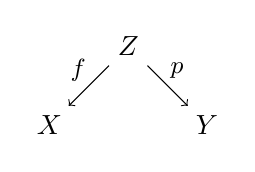
\begin{tikzpicture}[baseline=(current bounding box.center)]
      \node (X) at (-1,0){$X$};
      \node (Z) at (0,1){$Z$};
      \node (Y) at (1,0){$Y$};

      \draw (Z) edge[->] node[very near start,left=3pt]{{\small $f$}} (X);
;
      \draw (Z) edge[->] node[very near start,right=3pt]{{\small $p$}} (Y);
    \end{tikzpicture}
  \]
  with $p\in\mathcal E$; and
\item the composition of spans
    \[
      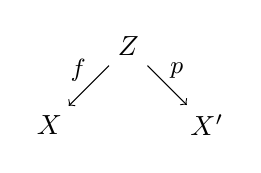
\begin{tikzpicture}[baseline=(current bounding box.center)]
        \node (X) at (-1,0){$X$};
        \node (Z) at (0,1){$Z$};
        \node (Xprime) at (1,0){$X'$};

        \draw (Z) edge[->] node[very near start,left=3pt]{{\small $f$}} (X);
        ;
        \draw (Z) edge[->] node[very near start,right=3pt]{{\small $p$}} (Xprime);
      \end{tikzpicture}
      \quad\text{and}\quad
      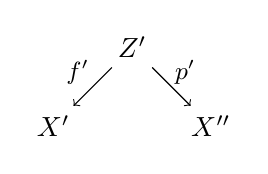
\begin{tikzpicture}[baseline=(current bounding box.center)]
        \node (X) at (-1,0){$X'$};
        \node (Z) at (0,1){$Z'$};
        \node (Xprime) at (1,0){$X''$};

        \draw (Z) edge[->] node[very near start,left=3pt]{{\small $f'$}} (X);
        ;
        \draw (Z) edge[->] node[very near start,right=3pt]{{\small $p'$}} (Xprime);
      \end{tikzpicture}
    \]
    is given by pullback---or more precisely as the outer span in the diagram
    \[
      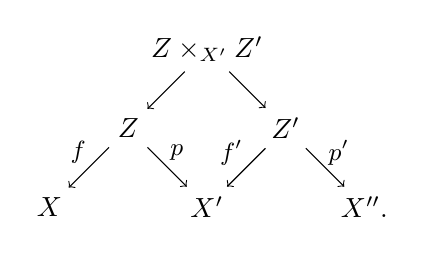
\begin{tikzpicture}[baseline=(current bounding box.center)]
        \node (X) at (-2,0){$X$};
        \node (Z) at (-1,1){$Z$};
        \node (Xprime) at (0,0){$X'$};
        \node (Zprime) at (1,1){$Z'$};
        \node (Xpprime) at (2,0){$X''.$};
        \node (pullback) at (0,2){$Z\times_{X'}Z'$};
        \node[rotate=-45] (pullbackcorner) at (0,1.6){{\large $\lrcorner$}};

        \draw (pullback) edge[->] (Z);
        \draw (pullback) edge[->] (Zprime);
        \draw (Z) edge[->] node[very near start,left=3pt]{{\small $f$}} (X);
        \draw (Z) edge[->] node[very near start,right=3pt]{{\small $p$}} (Xprime);
        \draw (Zprime) edge[->] node[very near start,left=3pt]{{\small $f'$}} (Xprime);
        \draw (Zprime) edge[->] node[very near start,right=3pt]{{\small $p'$}} (Xpprime);
      \end{tikzpicture}
    \]
\end{itemize}
Furthermore, the span category $\Span{\mathcal C}_{\mathcal E}$ has a symmetric monoidal structure, given informally by the categorical product on the underlying category $\mathcal C$. We refer to~\cites[][Definition 6.1.1]{Liu_Zheng2012}[][Definition~A.5.2 and Remark A.5.5]{Mann2022} for a precise construction of the span category and its symmetric monoidal structure.
\begin{defn}\label{defn:six-func}
  Let $(\mathcal C, \mathcal E)$ be a geometric setup and $\cA\in \CAlg(\Prlst)$ be some stable presentably monoidal category. 
  An \tdef{($\mathcal A$-linear) six-functor formalism} on 
  $(\mathcal C,\mathcal E)$ is a lax symmetric monoidal functor
  \[
    \mdef{\cD}\colon\Span{\mathcal C}_{\mathcal E}\longrightarrow
    \mathrm{Pr}^{\mathrm{L}}_{\mathcal A}.
  \]
\end{defn}
For the sake of exposition, the definition given here is more restrictive than the one in~\cite{Mann2022}, since we require $\mathcal D$ to take values in presentable categories.

\medskip

Note that any object $X\in\Span{\mathcal C}_{\mathcal E}$ has a canonical commutative algebra structure, with unit
\[
  \begin{tikzpicture}[baseline=(current bounding box.center)]
    \node (X) at (-1,0){$\pt$};
    \node (Z) at (0,1){$X$};
    \node (Xprime) at (1,0){$X$};

    \draw (Z) edge[->] (X);
    \draw (Z) edge[double equal sign distance] (Xprime);
  \end{tikzpicture}
\]
and multiplication
\[
  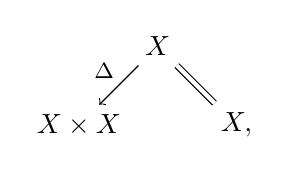
\begin{tikzpicture}[baseline=(current bounding box.center)]
    \node (X) at (-1,0){$X\times X$};
    \node (Z) at (0,1){$X$};
    \node (Xprime) at (1,0){$X,$};

    \draw (Z) edge[->] node[very near start,left=3.5pt]{{\footnotesize $\Delta$}} (X);
    \draw (Z) edge[double equal sign distance] (Xprime);
  \end{tikzpicture}
\]
see~\cite[Remark 3.13]{Scholze2025}. Unwinding the definition, we then see that a six-functor formalism on a geometric setup $(\mathcal C,\mathcal E)$ packages the following data:
\begin{itemize}
\item Since lax symmetric monoidal functors take commutative algebras to commutative algebras, we get a stable $\mathcal A$-linearly symmetric monoidal category $\mathcal D(X)\in\CAlg (\pPrl{\cA})$ for each object $X\in\mathcal C$;
\item By applying $\mathcal D$ to the span
  \[
    \begin{tikzpicture}[baseline=(current bounding box.center)]
      \node (X) at (-1,0){$X$};
      \node (Z) at (0,1){$Y$};
      \node (Xprime) at (1,0){$Y,$};

      \draw (Z) edge[->] node[very near start,left=3.5pt]{{\footnotesize $f$}}(X);
      \draw (Z) edge[double equal sign distance] (Xprime);
    \end{tikzpicture}
  \]
  we get a symmetric monoidal functor $f^*\colon \mathcal D(X)\to\mathcal D(Y)$ (called \tdef{pullback}) for each morphism $f\colon Y\to X$, together with a right adjoint $f^*\dashv f_*$ (called \tdef{pushforward});
\item By applying $\mathcal D$ to the span
  \[
    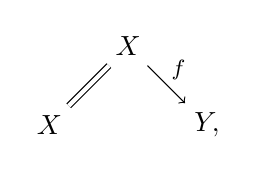
\begin{tikzpicture}[baseline=(current bounding box.center)]
      \node (X) at (-1,0){$X$};
      \node (Z) at (0,1){$X$};
      \node (Xprime) at (1,0){$Y,$};

      \draw (Z) edge[->] node[very near start,right=3.5pt]{{\footnotesize $f$}}(Xprime);
      \draw (Z) edge[double equal sign distance] (X);
    \end{tikzpicture}
  \]
  we get a functor $f_!\colon\mathcal D(Y)\to\mathcal D(X)$ (called \tdef{exceptional pushforward}) for each admissible morphism $f\colon Y\to X$ in $\mathcal C$ together with a right adjoint $f_!\dashv f^!$ (called \tdef{exceptional pullback});
\end{itemize}
Furthermore, this data satisfies
\begin{itemize}
\item \textbf{Base change:} For any cartesian square
  \[
    \begin{tikzcd}
      X' \arrow[r, "g'"] \arrow[d, "f'"] & X \arrow[d, "f"] \\
      Y' \arrow[r, "g"] & Y
    \end{tikzcd}
  \]
  in $\mathcal C$ with $f$ (and hence $f'$) admissible, 
  the Beck--Chevalley transformations $g^* f_* \xrightarrow{\sim} f'_* g'^*$ and $g_! f'^! \xrightarrow{\sim} f^! g_!$ are equivalences
\item \textbf{Projection formula:} For any admissible $f\colon Y\to X$, $A \in \mathcal D(Y)$, and $B \in \mathcal D(X)$, the canonical map $f_!(A \otimes f^* B) \to f_! A \otimes B$ is an equivalence.
\end{itemize}
\todo{Define (also for intuition of non-6FF-pilled reader): homology (ordinary and Borel--Moore), cohomology (ordinary and compactly-supported), properness, etc.}

\medskip

At first glance, it may seem that a six-functor formalism involves so much structure that it would be hard to construct one in practice. Nevertheless, \cite{Mann2022} gives a recipe (already implicit in \cite{Liu_Zheng2012}) for bootstrapping a six-functor formalism from a feasible amount of structure.\todo{This does not seem relevant to me}

Consider a geometric setup $(\mathcal C, \mathcal E)$, and suppose we are further given subclasses $\mathcal I, \mathcal P \subset \mathcal E$ such that
\begin{enumerate}[label=(\roman*)]
\item $\mathcal I$ and $\mathcal P$ contain equivalences and are under composition, base change, and diagonals.
\item If $f\in\mathcal I\cap\mathcal P$, then $f$ is $n$-truncated for some $n\geq 0$ \cite[Definition 5.5.6.8]{Lurie2009}. 
\item Every morphism $f \in \mathcal E$ admits a factorization $f = p \circ i$ with $i \in \mathcal I$ and $p \in \mathcal P$.
\end{enumerate}
Geometrically, we think of $\mathcal I$ as a class of ``open immersions'' and $\mathcal P$ as a class of ``proper maps''. Under this analogy, (ii) is then the statement that every admissible morphisms admits a compactification (cf.~Nagata compactifications in algebraic geometry, Stone--\v{C}ech compactifications in topology).
\begin{thm}[Liu--Zheng~\cite{Liu_Zheng2012}, Mann~\cite{Mann2022}]\label{thm:construction-IP}
  Let $(\mathcal C, \mathcal E)$ be a geometric setup, and let $\mathcal I$ and $\mathcal P$ be as above. Suppose we are given a functor
  \[
    \mathcal D_0\colon\mathcal C^{\mathrm{op}}\longrightarrow\CAlg (\pPrl{\cA}).
  \]
  If also
  \begin{enumerate}[label=(\roman*)]
    \setcounter{enumi}{3}
  \item the pullback $i^*$ admits a left adjoint $i_!$ for every $i\in\mathcal I$;
  \item the pushforward $f_*$ admits a right adjoint $f^!$ for every $f \in \mathcal P$; and
  \item the canonical map $i_!g_*\to f_*i'_!$ is an equivalence for every cartesian diagram
    \[
      \begin{tikzcd}
        U'\arrow[r,"i'"]\arrow[d,"g"]
        & X'\arrow[d,"f"] \\
        U\arrow[r,"i"]
        & X
      \end{tikzcd}
    \]
    in $\mathcal C$ with $f\in\mathcal P$ and $i\in\mathcal I$,
  \end{enumerate}
  then $\mathcal D_0$ admits a canonical extension to a six-functor formalism
  \[
    \mathcal D\colon\Span{\mathcal C}_{\mathcal E}\longrightarrow \pPrl{\cA}.
  \]
\end{thm}

\medskip

\todo{This is completely irrelevant}
It is often desirable to work with an $(\infty ,2)$-categorical enhancement of~\cref{defn:six-func}. Let $(\mathcal C,\mathcal E)$ be a geometric setup, and let $\mathcal I$ and $\mathcal P$ be subclasses of $\mathcal E$ satisfying conditions (i), (ii), and (iii) from the discussion preceding~\cref{thm:construction-IP}.
We can define an $(\infty ,2)$-category of spans $\sSpan{\mathcal C}_{\mathcal E,\mathcal I,\mathcal P}$ with the same objects and 1-morphisms as $\Span{\mathcal C}_{\mathcal E}$, and with 2-morphisms from $X\leftarrow Z\to Y$ to  $X\leftarrow Z'\to Y$ given by spans of spans
\[
  \begin{tikzpicture}[baseline=(current bounding box.center)]
    \node (X) at (-1.5,0){$X$};
    \node (Z) at (0,1.5){$Z$};
    \node (Zprime) at (0,-1.5){$Z',$};
    \node (W) at (0,0){$W$};
    \node (Y) at (1.5,0){$Y$};

    \draw (Z) edge[->] (Y);
    \draw (Z) edge[->] (X);
    \draw (Zprime) edge[->] (Y);
    \draw (Zprime) edge[->] (X);
    \draw (W) edge[->] node[near start,left=1.5pt]{{\footnotesize $f$}}(Z);
    \draw (W) edge[->] node[near start,left=1.5pt]{{\footnotesize $i$}}(Zprime);
  \end{tikzpicture}
\]
where $i\in\mathcal I$ and $f\in\mathcal P$. The symmetric monoidal structure on $\Span{\mathcal C}_{\mathcal E}$ extends to a symmetric monoidal structure on $\sSpan{\mathcal C}_{\mathcal E,\mathcal I,\mathcal P}$. We refer to Definition 4.10 and the discussion on page 50 in \cite{Cnossen_Lenz_Linskens2026} for the formal construction of  $\sSpan{\mathcal C}_{\mathcal E,\mathcal I,\mathcal P}$ and its symmetric monoidal structure.
\begin{thm}[Cnossen--Lenz--Linskens \cite{Cnossen_Lenz_Linskens2026}]
  Let $(\mathcal C,\mathcal E)$,$\mathcal I,\mathcal P\subseteq\mathcal E$, and $\mathcal D_0$ be as in~\cref{thm:construction-IP}. Then $\mathcal D_0$ admits a canonical extension to a lax symmetric monoidal 2-functor
  \[
    \mathcal D\colon\sSpan{\mathcal C}_{\mathcal E,\mathcal I,\mathcal P}^{\otimes}\too\mathcal P\mathrm r_{\mathcal A}^{L,\otimes_{\mathcal A}}.
  \]
\end{thm}

%%% Local Variables:
%%% mode: LaTeX
%%% TeX-master: "main"
%%% End:
